\documentclass{article}

\setlength{\textheight}{25.7cm}
\setlength{\textwidth}{16cm}
\setlength{\unitlength}{1mm}
\setlength{\topskip}{2.5truecm}
\topmargin 260mm \advance \topmargin -\textheight 
\divide \topmargin by 2 \advance \topmargin -1in 
\headheight 0pt \headsep 0pt \leftmargin 210mm \advance
\leftmargin -\textwidth 
\divide \leftmargin by 2 \advance \leftmargin -1in 
\oddsidemargin \leftmargin \evensidemargin \leftmargin
\parindent=0pt

\frenchspacing

\usepackage[english]{babel}
\usepackage{amsmath}
\usepackage{float}
\usepackage{graphicx}
\usepackage{subcaption}
\restylefloat{table}

\usepackage{listings}
\lstset{language=C++, showstringspaces=false, basicstyle=\small,
  numbers=left, numberstyle=\tiny, numberfirstline=false,
  stepnumber=1, tabsize=4, 
  commentstyle=\ttfamily, identifierstyle=\ttfamily,
  stringstyle=\itshape}

\title{Neural Networks: Assignment 2}
\author{Pepijn van Heiningen \\ \texttt{pvheinin@liacs.nl} \and Michiel Vos \\ \texttt{msvos@liacs.nl}}

\begin{document}

\maketitle

\section{Introduction}
The second assignment of the Neural Networks course consits of three tasks:\\
\begin{itemize}
\item Task 1: Function Optimization
\item Task 2: The XOR Problem
\item Task 3: Handwritten digit recognition
\end{itemize}

For the first task, we were given the Rosenbrock's function, and we were asked to test 5 different algorithms for finding the global minimum of this function. The purpose is to get an insight into the limitations of the classical gradient descent algorithm. 

%Task 2

%Task 3

\newpage
\section{Task 1: Function Optimization}
\subsection{Problem Description}
The Rosenbrock function is a function that is used as a performance test for optimization algorithms. The equation can be found in figure \ref{eq:rosen}. It has a global minimum at the point (1,1), where the value of $f = 0$. This is visualized in figure \ref{fig:rosenbrock}. \\

\begin{figure}[H]
\[f(x,y) = 100 * (y-x^2)^2 + (1 - x)^2\]
\caption{The Rosenbrock's function}
\label{eq:rosen}
\end{figure}

We were given the task to optimize the Rosenbrock function using five different algorithms, and subsequently compare their performance, in order to get an insight into the advantages, disadvantages and limitations of the different algorithms.\\

\begin{figure}[H]
	\centering
		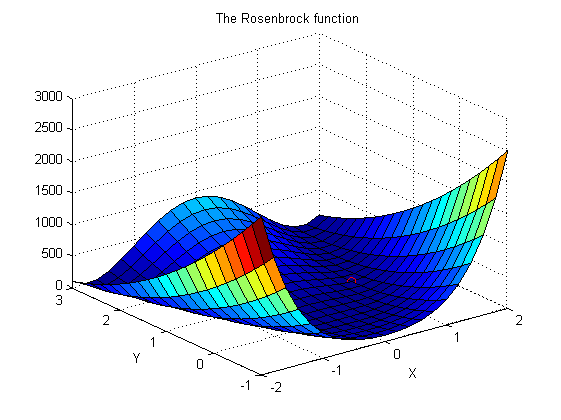
\includegraphics[scale=0.8]{rosenbrock.png}
	\caption{The Rosenbrock function, with minimal point}
	\label{fig:rosenbrock}
\end{figure}

The 5 different algorithms we tested are:
\begin{itemize}
\item Gradient descent
\item Gradient descent with line search
\item Scaled conjugate gradient
\item Conjugate gradient
\item Quasi-Newton
\end{itemize}

To get a good comparison between the algorithms, each algorithm was run 100 times.
We first generated 100 random points around (-1,1) as starting points. Each algorithm was started from the same random point.\\

\newpage
There were 4 different measures to compare the algorithms with:
\begin{itemize}
\item The average number of evaluations of $f$
\item The average number of evaluations of the gradient of $f$
\item The average run time of the algorithm
\item The average ``success rate''. 
\end{itemize}

Together these measures should provide a decent indication which algorithm performs better. Because some functions might be a lot more computationally expensive to evaluate than the Rosenbrock function, the number of evaluations of both the function and the gradient should be as low as possible. A run obviously shouldn't take too long, and it should have a high success rate. \\

The success rate is measured as reaching the minimum with an accuracy of 0.0001. This means that when the optimal point found by the algorithm is evaluated, the value of $f$ is smaller than 0.0001. Of course we would like to have an optimizer that gets a 100\% accuracy every time the algorithm is ran, but that is not always possible. 

\subsection{Implementation}
In figure \ref{fig:code} you can see the pseudo-code of the implemented algorithm.

\begin{figure}[h]
\begin{verbatim}
    starting_point = repmat([-1,1],100,1) + 0.5*randn(100,2);
    options = foptions;         % Standard options
    options(1) = -1;            % Turn off printing completely
    options(3) = 1e-8;          % Tolerance in value of function
    options(14) = 100;          % Max. 100 iterations of algorithm
    options(18) = 0.001;        % Learning rate    
    default_options = options;		
    functionList = {@graddesc, @graddesc, @scg, @conjgrad, @quasinew};
    for i = 1:100
        for j = 1:5
            options = default_options;
            if(j==1 || j==2)
                options(18) = 0.008;
            end
            if(j==2)
                options(7) = 1;
            end
            tic;
            [dump, options, dump, dump] = functionList{j}('rosen', starting_point(i,:), options, 'rosegrad');
            time = toc;
            results(i,j,1) = options(10);
            results(i,j,2) = options(11);
            results(i,j,3) = time;
            results(i,j,4) = options(8);
        end 
    end  
\end{verbatim}
\caption{Pseudo-code of task 1.}
\label{fig:code}
\end{figure}

As described in the assignment, we run the algorithms using 100 randomly generated starting points from the distribution \texttt{[-1, 1] + 0.5 * randn(1,2)}. 

We set the options of the algorithm to the default options, with a few changes, we set the tolerance of the function value to $1*10^{-8}$, the iterations to 100, and we use a different learning rate for the two gradient descent algorithms. The reasoning behind the value is described in section \ref{sec:experiments}.
%Options
%Partial derivatives of f

\subsection{Experiments}
\label{sec:experiments}
%Gradient descent experiments
In task $1.3$ we were asked to tune both gradient descent algorithms manually. We set the number of iterations to 100.000, and tested different values of the learing rate.

\begin{table*}[H]
	\centering
		\begin{tabular}{l|l|l}
		Learning rate & Gradient Descent & Gradient Descent with linesearch \\
		\hline
		0.05 & 0 & 0.054 \\
		0.01 & 0 & 0.058 \\
		0.008 & 0 & 0.058 \\
		0.005 & 0 & 0.056 \\
		0.001 & 0 & 0.038 \\
		0.0001 & 0 & 0.052 \\
		0.00001 & 0 & 0.050 \\
		\end{tabular}
\end{table*}
    
The values are averages over 500 runs. As you can see the optimal error is somewhere around a learning rate of 0.008, which is why we set the learning rate for the experiment to that value.

In order to acquire additional insights into how the algorithms work, we plotted the optimal points found after each iteration in the following plot.

\begin{figure}[H]
	\centering
	\begin{subfigure}[b]{0.45\textwidth}
		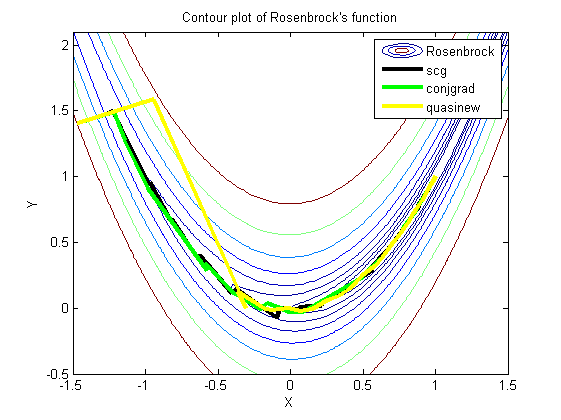
\includegraphics[width=\textwidth]{D:/Uni/nn2/rosenbrocktask1.png}
		\caption{Nadenken}
		\label{fig:rosenbrocktask1}
	\end{subfigure}
	\begin{subfigure}[b]{0.45\textwidth}
		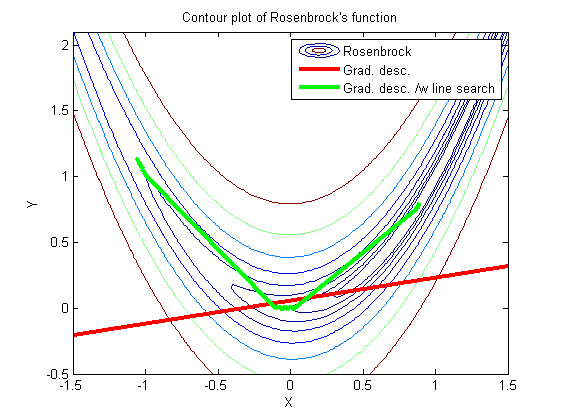
\includegraphics[width=\textwidth]{D:/Uni/nn2/rosenbrocktask12.png}
		\caption{Nadenken}
		\label{fig:rosenbrocktask1}
	\end{subfigure}	
\end{figure}

%Function 1:
%Average function evaluations: 101
%Average gradient evaluations: 100
%Average runtime: 0.0077814
%Average successrate: 0%
 %
%Function 2:
%Average function evaluations: 1816.93
%Average gradient evaluations: 98
%Average runtime: 0.19121
%Average successrate: 6%
 %
%Function 3:
%Average function evaluations: 0.47
%Average gradient evaluations: 0.7
%Average runtime: 5.3761e-05
%Average successrate: 100%
 %
%Function 4:
%Average function evaluations: 3.64
%Average gradient evaluations: 0.25
%Average runtime: 0.0003921
%Average successrate: 100%
 %
%Function 5:
%Average function evaluations: 0.69
%Average gradient evaluations: 0.22
%Average runtime: 7.9669e-05
%Average successrate: 100%

\subsection{Conclusions}

\newpage
\section{Task 2: The XOR Problem}
\subsection{Problem Description}

\subsection{Implementation}

\subsection{Experiments}

\subsection{Conclusions}

\newpage
\section{Task 3: Handwritten Digit Recognition with MLP}
\subsection{Problem Description}

\subsection{Implementation}

\subsection{Experiments}

\subsection{Conclusions}



\end{document}
